% %
% LAYOUT_E.TEX - Short description of REFMAN.CLS
%                                       99-03-20
%
%  Updated for REFMAN.CLS (LaTeX2e)
%
\documentclass[twoside,a4paper]{refart}
\usepackage{makeidx}
\usepackage{ifthen}
\usepackage{graphicx}
\usepackage{hyperref}
\hypersetup{
    colorlinks,
    citecolor=black,
    filecolor=black,
    linkcolor=blue,
    urlcolor=black
}
% ifthen wird vom Bild von N.Beebe gebraucht!

\def\bs{\char'134 } % backslash in \tt font.
\newcommand{\ie}{i.\,e.,}
\newcommand{\eg}{e.\,g..}
\DeclareRobustCommand\cs[1]{\texttt{\char`\\#1}}

\title{WARP User's Guide}
\author{Ryan M. Bergmann \thanks{ryanmbergmann@gmail.com} \\
Kelly L. Rowland \thanks{krowland@berkeley.edu}\\
v 1.0,  Oct 2015}

\date{}
\emergencystretch1em  %

\pagestyle{myfootings}
\markboth{WARP User's Guide}%
                {WARP User's Guide}

\makeindex 

\setcounter{tocdepth}{2}

\begin{document}

\maketitle

%\begin{abstract}
%
%This is the user guide for WARP.
%
%\end{abstract}

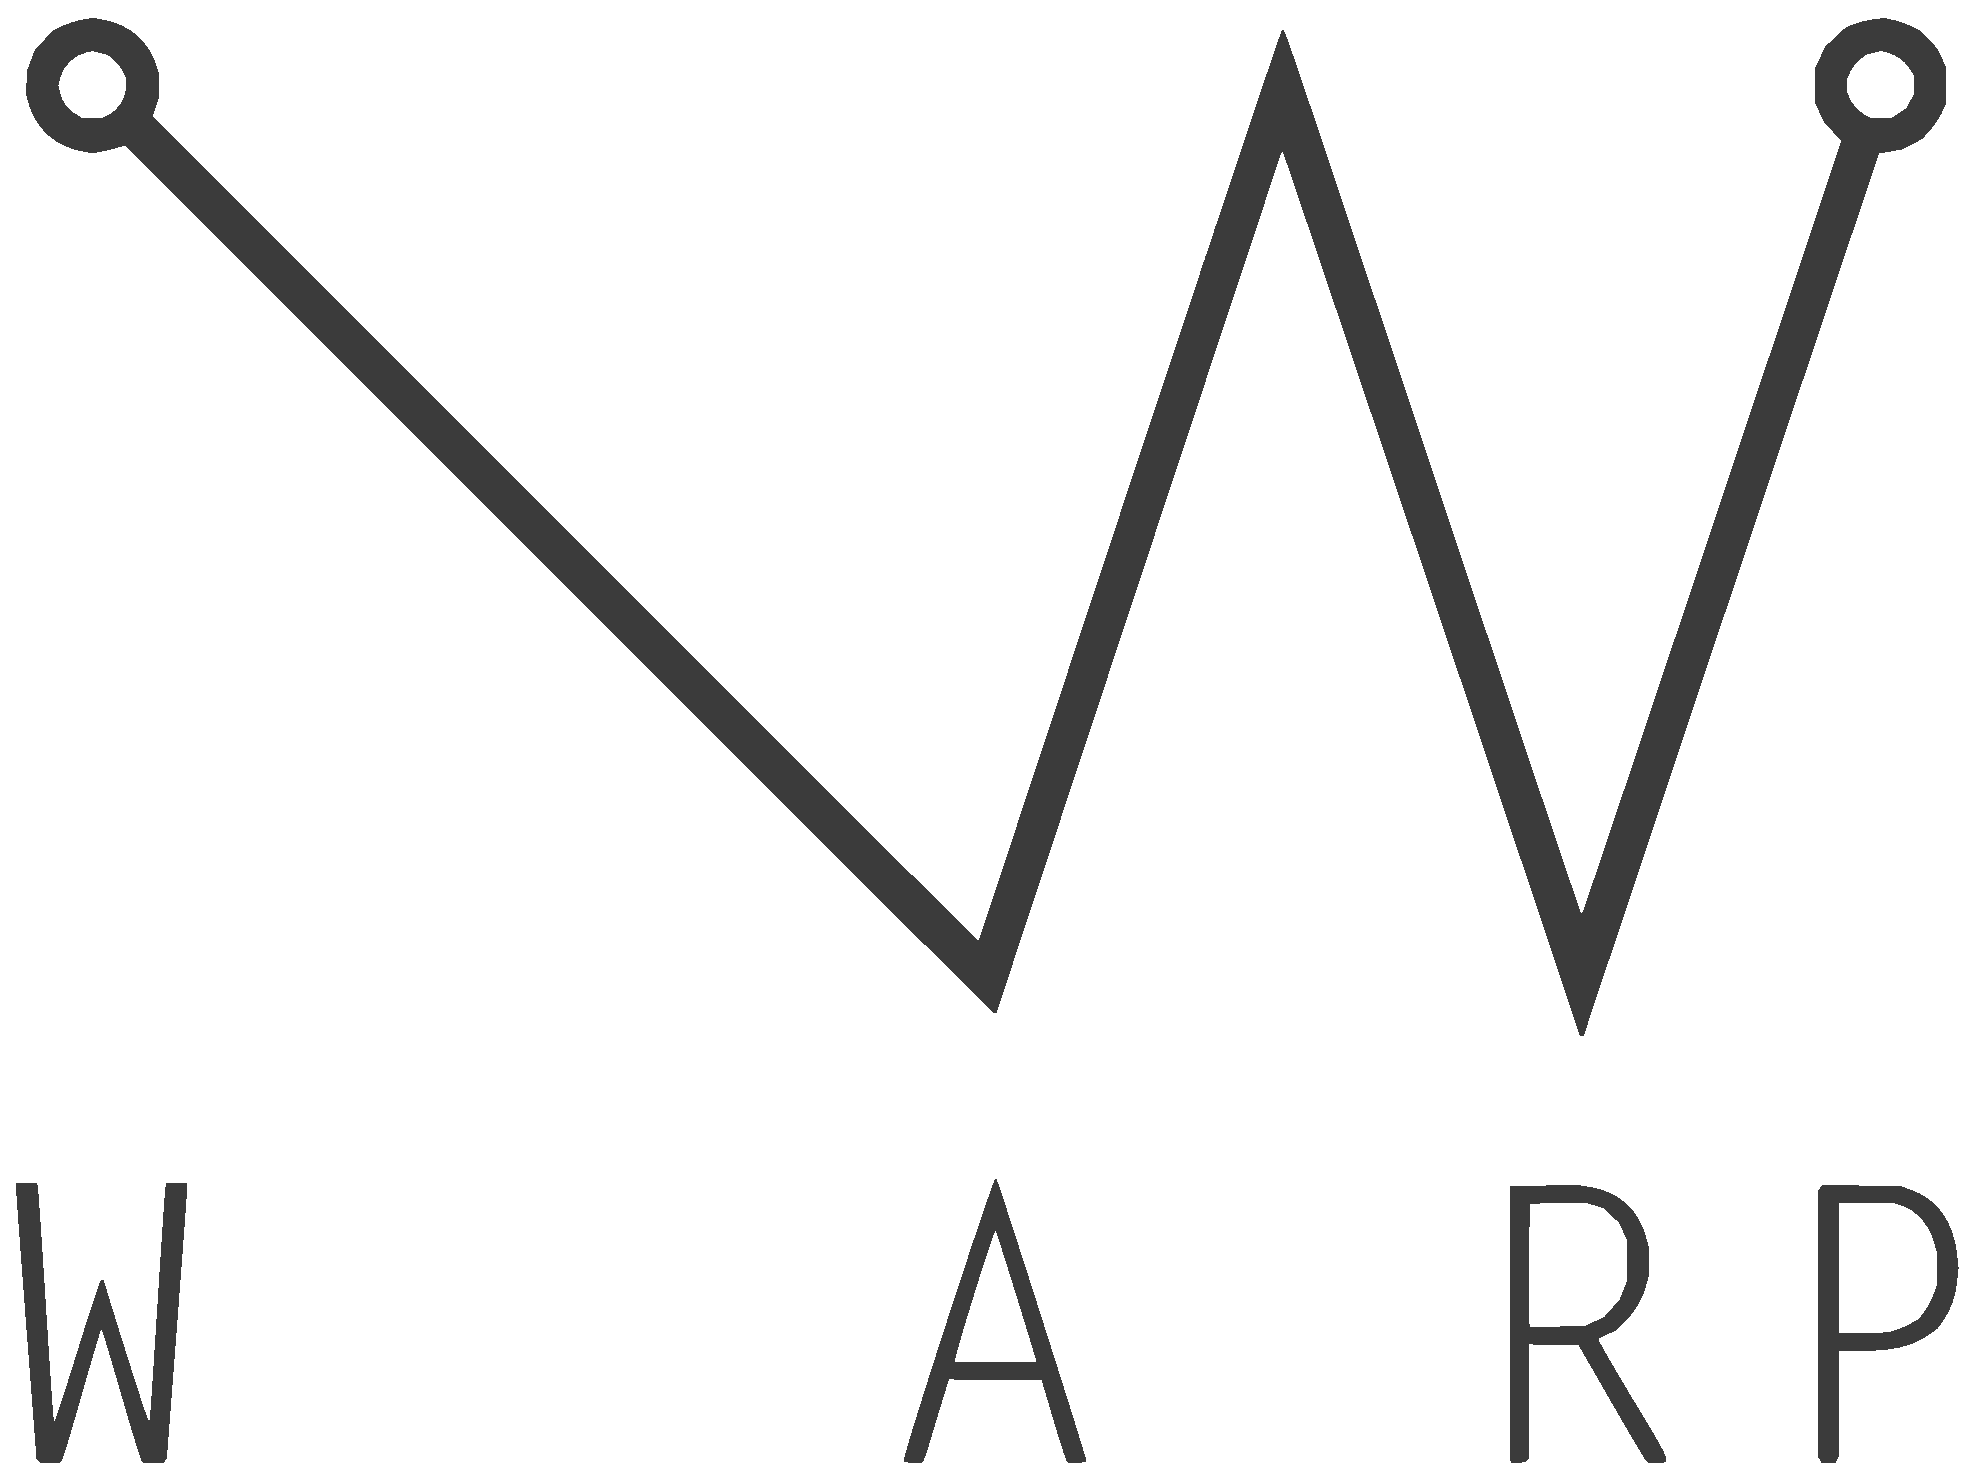
\includegraphics[width=\linewidth]{graphics/warp-vec.eps}

\vspace*{\fill} % this vertically centers the next paragraph

This user's guide is meant to introduce a user to the way in which WARP executes and how it's top-level functionality can be used to solve neutron transport problems.  For more detailed information about the algorithms WARP uses, please refer to article ``Algorithmic choices in WARP - A framework for continuous energy
Monte Carlo neutron transport in general 3D geometries on GPU'' in Annals of Nuclear Engineering (doi:10.1016/j.anucene.2014.10.039).

\vfill


\newpage
\tableofcontents
\newpage


%%%%%%%%%%%%%%%%%%%%%%%%%%%%%%%%%%%%%%%%%%%%%%%%%%%%%%%%%%%%%%%%%%%%

\section{An Introduction to WARP}

WARP is a C\texttt{++} library that contains a set of classes and data structures that allow Monte Carlo neutron transport to be performed using graphics processing units (GPUs).  It is written to scale well and execute efficiently on a single GPU.

Typical CPU codes track a single neutron life, from cradle to grave, marking its interactions along the way.  WARP does things a little differently.  WARP applies the main transport loop to an entire (preferably large) set of neutrons instead of a single neutron.  The parallelism in WARP comes from acting on many pieces of data concurrently instead of executing many tasks concurrently.


\begin{figure}[h!] 
  \centering
    \includegraphics[width=\textwidth]{graphics/datavtask.pdf}
     \caption{Data-parallel neutron trasport loop vs. a task-parallel transport loop for transporting N neutrons in parallel.  \label{datavtask} }
\end{figure}

\section{Dependencies of WARP}

WARP has the following dependencies:

\begin{description}

\item[C\texttt{++} compiler]\index{C\texttt{++} compiler}
	what about it?  Where can I get it?


\item[CMake]\index{CMake}$\ge$ 2.8.10 \\
CMake is ``an extensible, open-source system that manages the build process in an operating system and in
a compiler-independent manner."

CMake is free and can be downloaded here: \url{https://cmake.org/download/}.

Instructions for installing CMake on various operating systems can be found at 
\url{https://cmake.org/install/}.
  
\item[NVIDIA CUDA]\index{NVIDIA CUDA}$\ge$ 5.0 \\
	what about it?  Where can I get it?

\item[NVIDIA OptiX]\index{NVIDIA OptiX}$\ge$ 3.0.1 \\
	what about it?  Where can I get it?

\item[CUDPP]\index{CUDPP}$\ge$ 2.1 \\
	what about it?  Where can I get it?

\item[PyNE]\index{PyNE}$\ge$ ? \\
	what about it?  Where can I get it?

\item[SWIG]\index{SWIG}$\ge$ ? \\
	what about it?  Where can I get it?

\item[GoogleTest]\index{GoogleTest}$\ge$ ? \\
	what about it?  Where can I get it?

\item[ACE-formatted Nuclear cross section data]\index{ACE-formatted Nuclear cross section data}$\ge$ ? \\
	what about it?  Where can I get it?
        
\end{description}

\section{Building WARP}

WARP is compiled with CMake.

\begin{verbatim}
   how to use cmake to build warp
\end{verbatim}


\section{The Library Interface}

WARP has two interfaces available for use -- one in C\texttt{++} directly and one in Python.  The Python interface is a wrapper for the C\texttt{++} library, and basically gives access to identical methods.  For a complete list and detailed descriptions of all the library classes, methods, and data structures, please refer to the ``WARP\_API\_Reference.pdf'' which has been qutomatically generated from the source code with Doxygen and is included here.

\subsection{C\texttt{++}}

If using the C\texttt{++} interface, the user simply needs to compile WARP and specify which geometry
input to use at runtime. The syntax for compiling a WARP program are...



\begin{verbatim}
geom.set_datapath("/usr/local/SERPENT/xsdata/endfb7/sss_endfb7u.xsdir");
\end{verbatim}

Next, material and geometry information are specified. The material specification works as follows. The 
number of isotopes in the problem must be specified first, then the particular isotope(s) and their 
corresponding material fraction(s) assigned. Following that, a material density is specified and the 
material and its information are ``added" to the geometry object.

Information for tallying (the cell number in which to tally and the filename to which the tally data is written) is then defined.

Lastly, the geometry parameters are specified. The primitive type (cube, cylinder, hexagonal prism, or sphere) is noted and the number of the material with which the primitive will be filled is defined. The 
``mins", ``maxs", and ``origin" vectors are filled with the primitive's Cartesian minima, maxima, and origin, repsectively (in units of centimeters). The primitive is then added to the geometry object and a corresponding transform is also added to the geometry object. The outer cell is set and the boundary
condition (``1" for vacuum or ``2" for reflecting) is written.

An example of geometry and material specification for a bare plutonium sphere is shown below.

\begin{verbatim}
		n_topes = 1;
		std::vector<std::string> topes (n_topes);
		std::vector<float>    fracs (n_topes);

		// material information
		topes[0] = "94239.03c";
		fracs[0] = 1;      
		float    dens = 19.816;
		geom.add_material(1,1,n_topes,dens,topes,fracs);
		
		// run information
		tallycell = 999;
		filename = godivaname;
		tallyname = godivaname;
		tallyname.append(".tally");
	
		// geometry information
		type=3;
		material=1;
		mins[0]= -5.1;
		mins[1]= -5.1;
		mins[2]= -5.1;
		maxs[0]=  5.1;
		maxs[1]=  5.1;
		maxs[2]=  5.1;
		origin[0]=0.0;
		origin[1]=0.0;
		origin[2]=0.0;
		prim_id=geom.add_primitive(type,material,mins,maxs,origin);
		geom.add_transform(prim_id,999,0,0,0,0,0);

		geom.set_outer_cell(999,1);  // cell, BC  1=black, 2=specular
		geom.update();
\end{verbatim}

Finally, after the geometry and material input have been updated and checked by the code, parameters for how many neutron cycles to run are specified. A history object is instantiated with the number of
histories per cycle to run and the geometry object in which to run then. Then, a ``print level" and 
device (GPU) number are designated. The history is then initalized.

The user must specify whether to run in ``fixed-source" or ``criticality" mode, and the tally cell number
is sent to the history object. The code runs for a certain number of inactive cycles and then a number of
active cycles, where the numbers of cycles are designated by the user. Lastly, the file name to use for
tally information is sent to the history, the program is run, and the tally information is written out
upon successful completion.

Example syntax for setting up the history and cycle information is shown below. Here, the code is run in
``criticality" mode with 20 inactive cycles followed by 40 active cycles.

\begin{verbatim}
	whistory hist ( N , geom );
	hist.set_print_level(2);
	hist.set_device(0);
	hist.init();
	hist.print_xs_data();
	hist.print_materials_table();

	// converge fission source and run //
	hist.set_run_type("criticality");
	hist.set_tally_cell(tallycell);
	hist.set_run_param(40,20);  //run, skip
	hist.set_filename(filename);
	hist.run();
	hist.write_tally(0);
\end{verbatim}

Once the main function has been writen, it can be compiled and linked to the WARP shared library...

\begin{verbatim}
compile and link
\end{verbatim}

Which then creates an executable named ``warp'' in this case.  It takes two arguments here, a case name and the number of neutrons per batch.  This can be changed to a user's needs in any way one would normally write a C\texttt{++} program.  For example, the number of active and skipped cycles, an output file name, or the verbosity level could be passed in from the command line, etc.

\begin{verbatim}
./warp <geometry> <histories>
\end{verbatim}

where the four current geometry input options are ``godiva", ``homfuel", ``pincell", and ``assembly". If 
a different string is used or no string is specified, an error message is displayed, instructing the 
user to specify an appropriate condition. The last argument is the number of neutron histories to run in 
each cycle.

Program specifications are done in the ``main.cpp" file. After the instantiation of a geometry object, 
datapath ending in ``*.xsdir" must be designated as follows:

\subsection{Python}

The Python interface is very similar to the C\texttt{++} interface; the syntax differs only slightly.
Additionally, if the Python interface is used, the user is not restricted to the pre-programmed 
geometry and material configurations.

An example Python run file is shown below. The geometry and material configuration is the same as the
bare plutonium sphere example discussed above in the C\texttt{++} interface. Similarly, the code is set
to run in ``criticality" mode with 20 inactive and 40 active cycles of 100,000 neutron histories each.
The tally information will be written into a file called ``godiva.tally".

\begin{verbatim}
#! /usr/bin/env python
import warp

# init setup container
geom = warp.wgeometry()

# set datapath
geom.set_datapath("/usr/local/SERPENT/xsdata/endfb7/sss_endfb7u.xsdir")

# make materials
n_topes    = 1
prim_id    = 0
godivaname = "godiva"

topes = warp.String(n_topes)
fracs = warp.Float(n_topes)
mins    = warp.Float(3)
maxs    = warp.Float(3)
origin  = warp.Float(3)
topes[0] = "94239.03c"
fracs[0] = 1
dens = 19.816
geom.add_material(1,1,n_topes,dens,topes,fracs)

# run name stuff
tallycell = 999   #center pin
filename = godivaname
tallyname = godivaname
tallyname = godivaname+".tally"

# assembly geom
typ=3
material=1
mins[0]=-5.1
mins[1]=-5.1
mins[2]=-5.1
maxs[0]= 5.1
maxs[1]= 5.1
maxs[2]= 5.1
origin[0]=0.0
origin[1]=0.0
origin[2]=0.0
prim_id=geom.add_primitive(typ,material,mins,maxs,origin)
print prim_id
idx=geom.add_transform(prim_id,999,0,0,0,0,0)

# finalize geom and check
geom.set_outer_cell(999,1)
geom.update()
geom.check()
#geom.print_all()
geom.print_summary()


# init hist and run
hist = warp.whistory(100000,geom)
hist.set_device(0)
hist.init()
hist.print_xs_data()
hist.print_materials_table()
hist.set_run_type("criticality")
hist.set_tally_cell(tallycell)
hist.set_run_param(40,20)
hist.set_filename(filename)
hist.run()
hist.write_tally(0)
\end{verbatim}



\printindex

\end{document}
